\label{airy}
Ez a rész több különböző forrás, \cite{beals_wong_2010}, \cite{Albright_1977} és \cite{Vallee:2010:AFA} releváns eredményeinek rövid összegzése. Az Airy egyenlet
\begin{equation}
	\frac{d^2y}{dx^2} - xy = 0,
	\label{airy:airyeq}
\end{equation}
ennek az egyenletnek a megoldásai az Airy-függvények $\Ai(x)$ és $\Bi(x)$ lineáris kombinációi.

Az Airy-függvények szorosan kapcsolódnak a Bessel-függvényekhez. Ez jelentős mind az aszimptotikus alakjuk meghatározásához, mind a függvények numerikus kiértékeléséhez. A megoldást
\begin{equation}
	y(x) = x^{\frac{1}{2}}v\left(\frac{2}{3}x^{\frac{3}{2}}\right)
\end{equation}
alakban keresve a $x \geq 0$ tartományban a $v(x)$-re vonatkozó egyenlet a módosított Bessel-egyenlet $t=\frac{2}{3}x^{\frac{3}{2}}$ bevezetésével,
\begin{equation}
	t^2\frac{d^2v(t)}{dt^2} + t\frac{dv(t)}{dt} - \left(t^2 + \frac{1}{9}\right)v(t) = 0.
\end{equation}
A módosított Bessel-egyenlet nek van egy $\nu$ paramétere, a fenti egyenlet $\nu^2 = \frac{1}{9}$ esetnek felel meg. A $v(t)$-re vonatkozó egyenlet megoldásai az $I_{\frac{1}{3}}(t)$ és $I_{-\frac{1}{3}}(t)$ módosított Bessel-függvények lineáris kombinációi.
A két hagyományosan választott független lineáris kombinációk a
\begin{equation}
	\Ai(x) = \frac{\sqrt{x}}{3}\left(I_{-\frac{1}{3}}\left(\frac{2}{3}x^{\frac{3}{2}}\right)-I_{\frac{1}{3}}\left(\frac{2}{3}x^{\frac{3}{2}}\right)\right),
	\label{airy:ai+}
\end{equation}
\begin{equation}
	\Bi(x) = \sqrt{\frac{x}{3}}\left(I_{-\frac{1}{3}}\left(\frac{2}{3}x^{\frac{3}{2}}\right)+I_{\frac{1}{3}}\left(\frac{2}{3}x^{\frac{3}{2}}\right)\right).
	\label{airy:ai+}
\end{equation}
Az $x \leq 0$ tartományban hasonló,
\begin{equation}
	y(x) = (-x)^{\frac{1}{2}}v\left(\frac{2}{3}(-x)^{\frac{3}{2}}\right)
\end{equation}
alakban keresve a megoldást a $v(t)$-re kapott egyenlet ($t=\frac{2}{3}(-x)^{\frac{3}{2}}$) a Bessel-egyenlet, megint $\nu^2 = \frac{1}{9}$,
\begin{equation}
	t^2\frac{d^2v(t)}{dt^2} + t\frac{dv(t)}{dt} + \left(t^2 - \frac{1}{9}\right)v(t) = 0.
\end{equation}
Az $x=0$ pontban megkövetelt analitikusságnak megfelelően $x \geq 0$ esetén a választott lineáris kombinációk a
\begin{equation}
	\Ai(-x) = \frac{\sqrt{x}}{3}\left(J_{-\frac{1}{3}}\left(\frac{2}{3}x^{\frac{3}{2}}\right)-J_{\frac{1}{3}}\left(\frac{2}{3}x^{\frac{3}{2}}\right)\right),
	\label{airy:ai-}
\end{equation}
\begin{equation}
	\Bi(-x) = \sqrt{\frac{x}{3}}\left(J_{-\frac{1}{3}}\left(\frac{2}{3}x^{\frac{3}{2}}\right)+J_{\frac{1}{3}}\left(\frac{2}{3}x^{\frac{3}{2}}\right)\right),
	\label{airy:bi-}
\end{equation}
ahol $J_\nu(x)$ a Bessel-függvények.
\begin{figure}
	\centering
	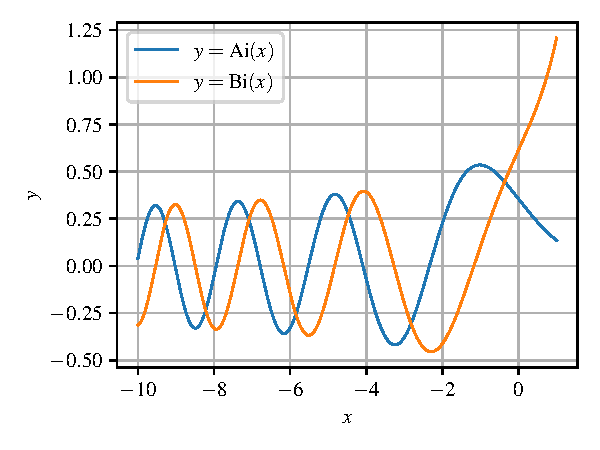
\includegraphics[scale=1]{./figs/airy.pdf}
	\caption[Airy-függvények]{$\Ai(x)$ és $\Bi(x)$ grafikonja.}
\end{figure}
Érdemes definiálni a
\begin{equation}
	\Ti(x) = \frac{\Ai(x)}{\Bi(x)}
\end{equation}
Airy-tangens függvényt.

Az aszimptotikus alakok megkaphatóak a Bessel-függvények aszimptotikus alakjából, 
\begin{equation}
	\Ai\left(-x\right) = \frac{1}{\sqrt{\pi}x^{1/4}}\cos\left(\frac{2}{3}x^{3/2} - \frac{\pi}{4}\right) + \mathcal{O}\left(x^{-5/4}\right),
	\label{airy:ai-approx}
\end{equation}
\begin{equation}
	\Bi\left(-x\right) = -\frac{1}{\sqrt{\pi}x^{1/4}}\sin\left(\frac{2}{3}x^{3/2} - \frac{\pi}{4}\right) + \mathcal{O}\left(x^{-5/4}\right),
	\label{airy:bi-approx}
\end{equation}
\begin{equation}
	\Ai(x) = \frac{1}{2\sqrt{\pi}x^{1/4}}e^{-\frac{2}{3}x^{\frac{3}{2}}}+\mathcal{O}\left(x^{-5/4}\right),
	\label{airy:ai+approx}
\end{equation}
\begin{equation}
	\Bi(x) = \frac{1}{ \sqrt{\pi}x^{1/4}}e^{ \frac{2}{3}x^{\frac{3}{2}}}+\mathcal{O}\left(x^{-5/4}\right).
	\label{airy:bi+approx}
\end{equation}
A $\Ti(x)$ definíciójába behelyettesítve \eqref{airy:ai-approx} és \eqref{airy:bi-approx} egyenleteket,
\begin{equation}
	\Ti\left(-x\right) = -\ctg\left( \frac{2}{3}x^{3/2} - \frac{\pi}{4} \right) + \mathcal{O}\left(x^{-5/4}\right).
	\label{airy:tiapprox}
\end{equation}

Az állapotok normájának kiszámításához szükség van az Airy-függvények szorzatának integráljára. \cite[A.16]{Albright_1977} szerint
\begin{equation}
	\int y^2\;dx = xy^2 - {y^\prime}^2,
	\label{airy:normintegral}
\end{equation}
ahol $y$ az Airy egyenlet tetszőleges megoldása. Ezen egyenlet segítségével tetszőleges kötött állapot normája meghatározható, azonban az esetleges szórási állapottok normálásához a Dirac-delta függvénnyel kapcsolatos relációra lesz szükség \cite{Vallee:2010:AFA} (3.108),
\begin{equation}
	\frac{1}{\alpha^2}\int_{-\infty}^\infty\Ai\left(\frac{x+a}{\alpha}\right)\Ai\left(\frac{x+b}{\alpha}\right)\,dx=\delta(a-b)
	\label{airy:delta}
\end{equation}

A Green-függvény meghatározása közben felmerül a Wronski-determinánsa az Airy-függvényeknek, ez \cite{NIST:DLMF} (9.2.7) szerint
\begin{equation}
	\mathcal{W} \{ \Ai(x), \Bi(x) \} = \Ai(x)\Bip(x) - \Bi(x)\Aip(x) = \frac{1}{\pi}.
	\label{airy:wronski}
\end{equation}








